\subsection{CPU, Scheduling, and OS Services}

\subsubsection{Measurement overhead}

As we are microbenchmarking, the overhead of the measurement tools that we
choosed may influence our results. Thus we need to know the cost of reading
the clock and since we are using loops for averaging the results of the tests, we
also need to know the overhead caused by these loops.

\paragraph{Methodology}
We are using the \emph{rdtsc} assembly instruction to do the measurement.
The \emph{rdtsc} instruction allows us to read the \emph{Time Stamp Counter}
which is a 64 bit counter containing the number of cycles elapsed since his
reset.
In terms of implementation, the instruction is integrated in the code using
inline assembly and is called using a function which is inlined to avoid the
overhead of the procedure call and the stack frame creation.
To measure the cost of the reading clock operation, we measured the result between
two calls and repeated the operation 100,000 times.\\

The loop overhead has been measured with 100,000 iterations.

\paragraph{Predictions}
The operations between the two rdtsc call are basicly a copy from the result
which are stored in the eax and edx register to the main memory, a binary shift
and a binary OR on the two variables.
As the cache may be hited, it's basicly two cache write, around 10 cycles, and
the cost of the second rdtsc call.\\

As all optimization are turned off, the cost of a loop iteration is basicly a
load from memory, an incrementation, a store to memory, a comparaison and a
jump.
The cache will probably be hited, thus the cost of memory operations will be low.
The total cost may be around 15 cycles if we count 10 cycles for the memory
latency and 1 cycle for operation such as incremention, comparaison and
jump.\\

There is no software overhead in any of these operations.

\paragraph{Results}

\begin{center}
\begin{tabular}{| l | l | l | l | l |} \hline
Operation 			& Hardware cost 	& Software cost 	& Prediction	& Measured \\ \hline
Reading the clock 	& 25 cycles		& 0 cycles			& 25 cycles 	& 58.555 cycles \\ \hline
Loop 				& 15 cycles 		& 0 cycles 		& 15 cycles 	& 12.487 cycles \\ \hline
\end{tabular}
\end{center}

Compared to the actual result, our estimates are too low for the reading time, due to the cost of the memory write operation which is
higher than excepted.
It seems that we fill the cache latency due to the dependency of the data
avoiding the effective use of the pipelining.
This hypothesis on the memory write operation cost is due to the fact that on long run,
the result is lowered to aproximatly 30 cycles after 50,000 iterations.
We choosed to report the average of a run which did not show this reduction in
the cost because it seems more accurate (i.e. we will call rdtsc once for each
loop).\\

Our estimates are in the good range for the loop.

\paragraph{Success of Methodology}
Our result for the reading time are varying but we have an average result. As
the overhead will be accounted only once for many iterations, this will not
cause more problem.\\

The result for the loop overhead seems accurate.

\subsubsection{Procedure call overhead}
\paragraph{Methodology}
We defined seven functions with different number of arguments to test the
cost of a procedure call and the overhead of an argument.
Each procedure call is made 100,000 time in a loop and the total is measured.
The cost per loop cycle is then calculated and the overhead of the loop is
removed.

\paragraph{Predictions}
On x86-64 a procedure call is composed off :
\begin{enumerate}
\item Moving the arguments into specific registers (for the 7 first arguments)
\item Calling the procedure, that is jumping to the beginning of the procedure
\item Creating a new stack frame, that is saving the previous stack pointer and
moving the stack pointer into the begin stack pointer
\item Destroying the stack frame
\item Restoring the instruction pointer
\end{enumerate}

The latency of the memory operations may be hidden due to pipelining.
The procedure call should normally be predicted by the branch prediction part of
the processor avoiding stall of the processor.
The architecture of the Intel Sandy Bridge is very complex, making prediction is
really difficult.
We can guess that the procedure call will take about 10 cycle and that each
argument will cause a cost of one cycle due to the new register access.

\paragraph{Results}
\begin{center}
\begin{tabular}{| l | l | l | l | l |}
\hline
\# of args & Hardware cost & Software cost & Prediction & Measured \\ \hline
0 & 2  & 8   & 10  & 14.471 cycles \\ \hline
1 & 2  & 9   & 11  & 14.471 cycles \\ \hline
2 & 2  & 10  & 12  & 14.455 cycles \\ \hline
3 & 2  & 11  & 13  & 14.462 cycles \\ \hline
4 & 2  & 12  & 14  & 14.461 cycles \\ \hline
5 & 2  & 13  & 15  & 14.461 cycles \\ \hline
6 & 2  & 14  & 16  & 14.456 cycles \\ \hline
7 & 2  & 15  & 17  & 16.518 cycles \\ \hline
\end{tabular} \\
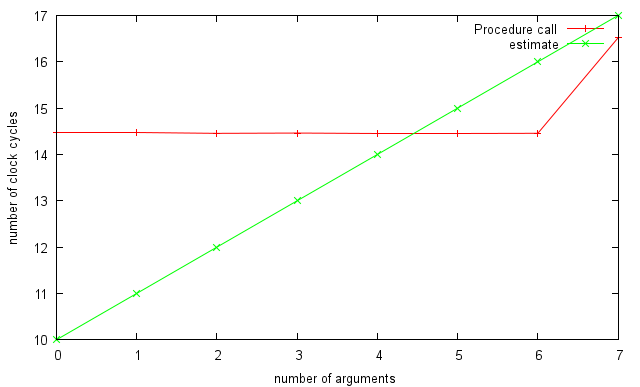
\includegraphics[scale=0.8]{procCallImage}
\end{center}


\paragraph{Accuracy of Estimates}
The results are low as predicted. Apparently the cost of accessing one more argument is too low to be detected. Only when the function take 7 aguments, which cannot all fit into the registers. The 7th argument is put into the stack and the cost for doing that turns out to be about 2 cycles.

\paragraph{Success of Methodology}







\subsubsection{System call overhead}
\paragraph{Methodology}
We choosed the getpid() system call to test the overhead for a minimal system
call as it's supposed to be the least expensive system call.
We then ran it 10,000 times to get an averaged result.

\paragraph{Predictions}
System call are excepted to be more expensive than simple procedure call as they
produce a context switch.
The state of the process need to be saved and a kernel thread must be launched.
The way back need also to be done.
We except something like 400 cycles for each context switch, so a total of about 800 cycles.

\paragraph{Results}

\begin{center}
\begin{tabular}{| l | l | l | l | l |}
\hline
Operation & Hardware cost & Software cost & Prediction & Measured \\
\hline
Context switch (1st run) & 200 cycles & 600 cycles & 800 cycles & 5000 cycles\\
\hline
Context switch (average) & 200 cycles & 600 cycles & 800 cycles & 750 cycles\\
\hline
\end{tabular}
\end{center}

The first call is always slow, probably due to the need to read kernel code and
kernel memory which are not in cache.
The following calls are going faster probably due to branch prediction and
cache.
We can see that system calls are much expensiver than procedure calls as
excepted.

\paragraph{Accuracy of Estimates}
We didn't predicted that the first run would be that slow.
The following

\paragraph{Success of Methodology}


\subsubsection{Task creation time}
\paragraph{Methodology}
We measured the time to create process and thread seperately. After that, we compared them to each other to verify our measurement. When a new process is created, the page tables and stack frame are copied. While for creating a kernel thread, less information are required to get copied because of the fact that a lot of the resource in thread are shared with the main thread.
We used the system call fork() for creating a new process and record the number of cycles from before the fork() is called to the point waitid() get back from the new process. And for the newly created process, we called \_exit() to immediated exit after creation.
Similarly, we used the solaris implementation, which is thr\_create() for cloning thread. At first we used pthread\_create() fuction for thread creation operation. We replaced it with thr\_create() later because it is not meant for Solaris system, which is not as accurate when we are doing the measurement of the whole Solaris OS. Right after the creation of the thread, we used thr\_join() to wait for the termination of itself.
At the same time, we measured the time for the program to create process and threads for the first time only as well, for loading the functions we used in this measurement into the cache.
The creation overhead has been measured with 100,000 iterations.


\paragraph{Predictions}

As mentioned earlier, the thread has less data to copy than process do. Meanwhile, the process creation is using system call instead of function call, which envolves two context switching time. We predict that process creation is about 10000 cycles taking longer than thread creation 8000 cycles.






\paragraph{Results}
\begin{center}
\begin{tabular}{| l | l | l | l | l | l |}
\hline
Operation & H/W cost & S/W cost & Prediction & Measured average & Measured first creation \\
\hline
fork() process 		& 20  & 10000  	& 10000 & 1198519.65 cycles & 2257852 cycles\\ \hline
thr\_create() thread 	& 20  & 8000	& 8000  &  157433.27 cycles & 2273593 cycles \\ \hline
\end{tabular}
\end{center}


\paragraph{Accuracy of Estimates}
The measurement result mostly fits our prediction besides the fact that the number of cycles are way bigger than what we expected.
\paragraph{Success of Methodology}
For testing the overhead of creating a new process, we simply called fork(). It turned out that it takes about 750,000 clock cycles for creating it without caching and less than 500,000 with caching.While for the overhead of creating a new thread, we simply called pthread\_creat(). It turned out that it takes about 2000,000 clock cycles for creating it without caching and less than 80,000 with caching.
The fact thread creation without caching is taking way longer time than the one for process creation doesn't really make sense to us right now, and we will look into that later as the project goes. But considering that thread creation does't envolve memory alloction, the average case for thread creation is generally faster then the one for process creation.


\subsubsection{Context switch time}
\paragraph{Methodology}
\paragraph{Predictions}
\paragraph{Results}

\begin{center}
\begin{tabular}{| l | l | l | l | l |}
\hline
Operation & Hardware cose & Software cost & Prediction & Measured \\
\hline
\end{tabular}
\end{center}

\paragraph{Accuracy of Estimates}
\paragraph{Success of Methodology}
We measured the context switching overhead for both processes and threads. The way we define context switching is by creating a child process/thread and make the child do some task and return back to the parent. The overhead of such context switching is going to be the time start from the creation of the child to the time execution gets back to the parent process/thread excluding the time for child to execute. We only tested the context switching within 2 different processes.
//***TODO actual result

